\documentclass{report}
\usepackage[utf8]{inputenc}
\usepackage{natbib}
\usepackage{graphicx}
\usepackage[pagestyles]{titlesec}

\title{Design Document}
\author{AmorosiniCasaliFioravanti}
\date{December 2019}

\titleformat{\chapter}[display]{\normalfont\bfseries}{}{0pt}{\Huge}
\newpagestyle{mystyle}
{\sethead[\thepage][][\chaptertitle]{}{}{\thepage}}
\pagestyle{mystyle}

\begin{document}

\maketitle

\chapter{Introduction}
\section{Purpose}
While the RASD presented a general view of the SafeStreets appliction and its features, this document aims to further analyze the system's design and architecture, by describing for each of its components their runtime behaviour, integration, interfaces, implementation and testing plans.
This document is mainly intended to be used by the test and development teams as a guidance in the development process, but also to prevent structural degradation during maintainance and extension phases. Nonetheless, the document is also addressed to all the stakeholders who are interested in supervising the development process.

\section{Scope}
SafeStreets: an application that aims to improve the safety of urban areas by giving its Users the possibility to report traffic violations to Authorities. Users are logged in either as Citizen, those who report the violations, and Authorities, those who are notified about newly reported violations and are supposed to take action on them.\\
The system is in charge of collecting all the Reports, storing them, and notifying the Authorities about them. The stored Reports are then used to build statistics, find unsafe areas, and compute suggestions on how to improve the safety of such areas. The system can also communicate local Municipalities' Systems in order to retrieve information about accidents and iussued traffic ticket: in this case some of the above functions are enhanced, and some new functions are enabled (g.e computing statistics on traffic ticked).\\
\newline
Further information about the scope of the application can be found in the Chapter 1 of the RASD.

\section{Definitions, Acronyms and Abbreviations}
\subsection{Definitions}
\begin{itemize}
    \item \textit{Client}: a piece of computer hardware or software that accesses a resource or a service made available by a Server.
    \item \textit{Server}: a device or a computer program that provides resources or functionalities to other programs or devices.
    \item \textit{Reverse Proxy}: particular proxys that are responsible of forwarding requests to one or more Servers which will handle it.
    \item \textit{Firewall}: a network security systems that monitors incoming and outcoming network traffic, applying predefined predefined security rules.
    \item \textit{Port}: %To remove if undefined
\end{itemize}
\subsection{Acronyms}
\begin{itemize}
    \item \textbf{RASD}: \textit{Requirement Analysis and Specification Document}, the document in which all the requirements and goals of the application are throughly described.
    \item \textbf{API}: \textit{Application Programming Interface}, interface, or communication protocol between Client and Server intendend to simplify the building of the Client-side software.
    \item \textbf{OCR}: \textit{Optical Character Recognition}, software dedicated to the detection of characters contained in a document and to their transfer to digital text that can be read by a machine. In this context, OCR will be used to read license plates.
    \item \textbf{UML}: \textit{Unified Modeling Language}, is a standard visual modeling language intended to be used for analysis, design, and implementation of software-based systems.
    \item \textbf{GPS}: \textit{Global Positioning system}, technology widely used to get the user's position.
    \item \textbf{DBMS}: \textit{Data Base Management system}, software that provides organized space memory to store information.
    \end{itemize}
\subsection{Abbreviations}
\begin{itemize}
    \item {[R$_{i}$]}: i-th requirement.
    \end{itemize}
\section{Reference Documents}
\begin{itemize}
    \item Specification document: \textit{SafeStreets Mandatory Project Assignment.pdf}.
    \item Requirement Analysis and Specification Document: \textit{RASD.pdf}.
\end{itemize}
\section{Document Structure}
This document is presented as it follows:
\begin{enumerate}
    \item \textbf{Introduction} presents a general overview, the scope and the purpose of the document.
    \item \textbf{Architectural Design} shows the main components of the system and their relationships. This section will also discuss the arichitectural choices of the design process.
    \item \textbf{Algorithm Design} presents and discusses the algorithms that will enable the system's functionalities.
    \item \textbf{User Interface Design} provides some further details on the user interface defined in the RASD.
    \item \textbf{Requirement Traceability} maps all the functional requirements defined in the RASD over the components that will accomplish them.
    \item \textbf{Implementation, Integration and Testing Plans} shows the order in which the implementation and the integration of the components will occur, and how the testing phase will be carryed out.
    \item {\textbf{Effort spent}} displays the time spent writing this document by each member of the team.
\end{enumerate}
\chapter{Architectural Design}
\section{Overview}
In this chapter we are going to discuss the architectural structure of the System. In Figure 1 is represented an high-level view of the components and their interactions. The details are explained in the next sections.
\begin{figure}[!ht]
	\begin{center}
	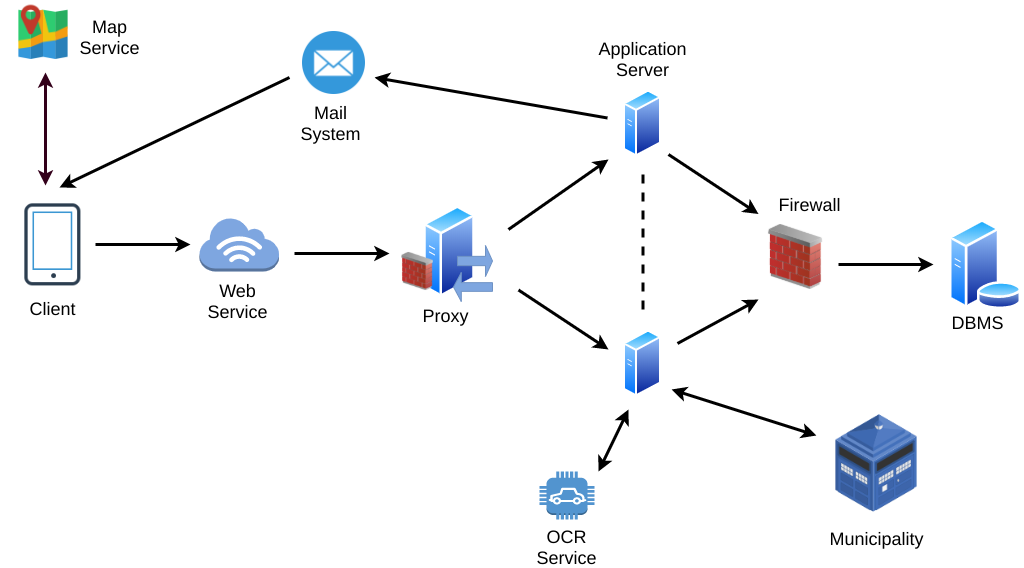
\includegraphics[width=\textwidth]{img/HighLevelOverview.png}
	\end{center}
	\caption{Overview of the System.}
\end{figure}

\section{Component view}

\section{Deployment view}

\section{Runtime view}

\section{Component interfaces}

\section{Selected architectural	styles and patterns}
The following architecture are used for the structure of the System in order to provide all the services of SafeStreets application.
\subsection{Client-Server Architecture}
In this structure there are two main role with different duties, the client uses data and services offered by the server.
The server stores all data in order to provide them to the client.\\
\textbf{Motivations:} this structure dues to several advantages. Server can be replicated to have more scalability. 
Accessibility: users can use the services without hte need for a specialized device or client.
The security is granted because the server allows only registered user to consult data.
Furthermore, it is easy to update, replace, repair, move a server without affecting clients.
\subsection{Three-tiered Architecture}
This type of architecture is a client-server architecture where three tiers are phisically separated.
\begin{itemize}
	\item The \textit{presentation tier} provide an interface to allow the user to consult data and result of services executed in a different layer. 
	It is the top-most tier and the only one accessible from the client.
	\item The \textit{application tier} executes the logic of the application throw functions that elaborate data. 
	The reverse proxy is needed to handle the client requests and to balance the workload, the requests are forwarded to 
	the application serves in order to provide the right data.
	\item The \textit{database tier} includes the data persistence mechanisms and the data access layer that encapsulates 
	the persistence mechanisms and exposes the data.
\end{itemize}
\textbf{Motivations:} A multi-tier application architecture provides a model with several advantages: developers can create flexible and reusable 
applications and acquire the option of modifying or adding a specific layer, instead of reworking the entire application.

\begin{figure}[!ht]
	\begin{center}
	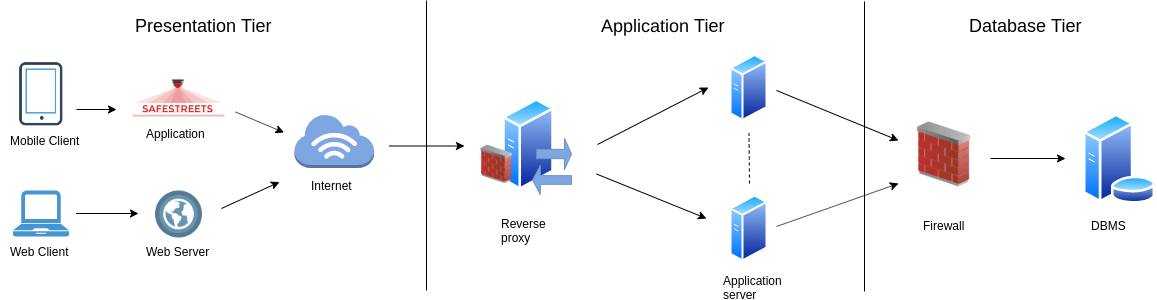
\includegraphics[width=\textwidth]{img/TiersArchitecture.png}
	\end{center}
	\caption{Overview of the System.}
\end{figure}

\subsection{MVC Design Pattern}
Model-View-Controller is a software design pattern particulary usefull to develope user interfaces. Indeed, this pattern is used for the frontend implementation of the application. 
It divides the program logic in three interconnected elements: \textit{model} that directly manages data and rules of the application, \textit{view} which handles any representation of data, \textit{controller} that 
accepts input and converts it to commands for the model or view. This is done to separate internal representations of information 
from the ways information is presented to and accepted from the user. \\
\textbf{Motivations:} MVC allows full encapsulation of object. This means that each component can be changed without creating issues to other components.
Furthermore, with MVC developers are able to work in parallel on different components without blocking another.

\end{document}